\chapter{Discussion}
\label{chap:discussion}
In this chapter we will discuss the results presented in \autoref{chap:results}. We will also discuss the limitations of the current setup and possible improvements.

\section*{Laser heating}
As mentioned in \autoref{chap:results}, the particle lost its magnetization when irradiated with the laser at low pressures ($<\qty{1}{\milli\bar}$). Decreasing the laser intensity also resulted in a smaller SNR. Due to this tradeoff a decision was made to only use camera measurements at low pressure. A comparison between the two methods will follow. Besides the total loss of magnetization we are also not sure how well the particle retains its magnetization over time. In addition to this we are also not sure what the resulting magnetization is since we do not reach the saturation field. A future project will focus on designing a device that can fully saturate the particle.

\section*{Damping at low pressures}
We observed a limit in the Q-factor for pressures below \qty{1E-2}{\milli\bar}. Attempts to model this have been unsuccessful and do not match the experimental results (see \autoref{tab:dissipation}). Proper modelling of the dissipation should involve a time dependent simulation in COMSOL instead of using a Lorentz term. The main reason for this is that a displacement of the particle brings it closer to its surrounding as such any effects due to the magnetization of the particle will be stronger. Another source of damping could be eddy currents inside the particle itself. In addition to this we should consider additional sources of damping, such as noise from the electronics or anisotropy (differences in magnetization) inside the particle\cite{millen}. Recent works also discuss eddy currents in more detail, including how they would behave in superconductors\cite{fuwa_stable_2023,gutierrez_latorre_chip_2023}.

Another explanation for the damping is that the pressure inside the trap is not in equilibrium with the pressure in the chamber. This would result in a higher pressure inside the trap compared to the vacuum chamber. As a result a higher damping rate than expected is observed. One way to test this hypothesis would be to see if the damping rate changes over time when the chamber pressure is kept at a low value.

A statistical test (see \autoref{tab:gamma-t-test}) suggests that the damping of the \zmode is significantly higher than the damping of the \xmode and \ymode. This might shed light on the origin of the damping, but it may also be caused by non-linear effects in the trap. Due to the difficulty of observing the \zmode, we needed quite strong driving forces which can cause non-linear effects. Improvements in the detection of the particle position will allow us to measure the \zmode at lower driving forces.

\section*{Laser v.s. camera readout}
The disadvantages and advantages of the camera and laser readout are summarized in \autoref{tab:laser-vs-camera-readout}.

\begin{table}[h]
    \begin{tabularx}{\textwidth}{XX}
        \toprule
        Camera readout & Laser readout \\
        \midrule
        \begin{itemize}[left=0pt,topsep=0pt,label=\textcolor{green}{\texttt{+}}]
            \item Immediate visual feedback about the behaviour of the particle;
            \item SNR only dependent on the contrast of the particle;
        \end{itemize} \begin{itemize}[left=0pt,topsep=0pt,label=\textcolor{red}{\texttt{-}}]
            \item Limited sample rate (roughly \qty{400}{\fps}) so observation of the librational modes is not possible;
            \item No `real' lock-in measurements possible;
            \item Live analysis is not possible;
        \end{itemize} & \begin{itemize}[left=0pt,topsep=0pt,label=\textcolor{green}{\texttt{+}}]
            \item High sample rate that is only limited by the gain bandwidth product of the photodiode;
            \item `Real' lock-in measurements possible by connecting the photodiode to a lock-in amplifier;
        \end{itemize} \begin{itemize}[left=0pt,topsep=0pt,label=\textcolor{red}{\texttt{-}}]
            \item SNR is dependent on the laser intensity, background light and electronic noise;
            \item No immediate visual feedback about the behaviour of the particle;
            \item High laser intensity can cause the particle to lose its magnetization;
        \end{itemize} \\
        \bottomrule
    \end{tabularx}
    \caption{Advantages and disadvantages of camera and laser readout.}
    \label{tab:laser-vs-camera-readout}
\end{table}

In the future laser readout is key to properly study the $\gamma$ and $\beta$ modes at low pressures. The idea is to move to an interferometric setup to measure the position of the particle. This has a higher SNR if done correctly. In addition to this we are also investigating the use of NV centres in diamond to measure the position of the particle. An additional advantage of NV centres is that they may also allow for sideband cooling.

\section*{Lorentzian fits}
To obtain the data in \autoref{fig:xyz-mode-dependence-on-trapping-frequency-1mbar} we fitted the peaks in our data with a Lorentzian. This was done to obtain the Q-factor of the peaks. It is however better to fit all peaks at once instead of individually. The reason we did not do so is that the spectra were not very clean. An example of this is the fact that there was crosstalk between the horizontal and vertical spectra. A more careful analysis could properly rotate the spectra to avoid this crosstalk. This might make it easier to do a single fit per spectra instead of 2 separate fits.

\section*{Trapping at low pressures}
Qualitatively we found it to be very hard to trap the particle at low pressures ($<\qty{1}{\milli\bar}$) when starting from an untrapped state. It is likely that more damping is needed to dissipate the energy of the particle or active feedback to trap the particle. Potentially we can artificially introduce damping by adding white-noise to a nearby coil. White-noise increases the damping rate\cite{millen}. This is something that should be investigated further.

\section*{Loss of levitation}
A major source of confusion (and frustration) was the sudden loss of levitation. For long periods of time our particle was easily trapped without major issues. However, just before the Christmas holiday it became very difficult to trap. We had previously seen that heating can cause the particle to lose its magnetization, but didn't appear to be the case as it still responded to the magnetic field. An attempt was mode to remagnetize the particle which did not matter much. Using an optical microscope we noted a black `smut' in and around the trap. This was further confirmed using SEM measurements. This `smut' was not found on earlier images before we used the trap. See \autoref{fig:smut-optical-microscope}.

\begin{SCfigure}[50]
    \centering
    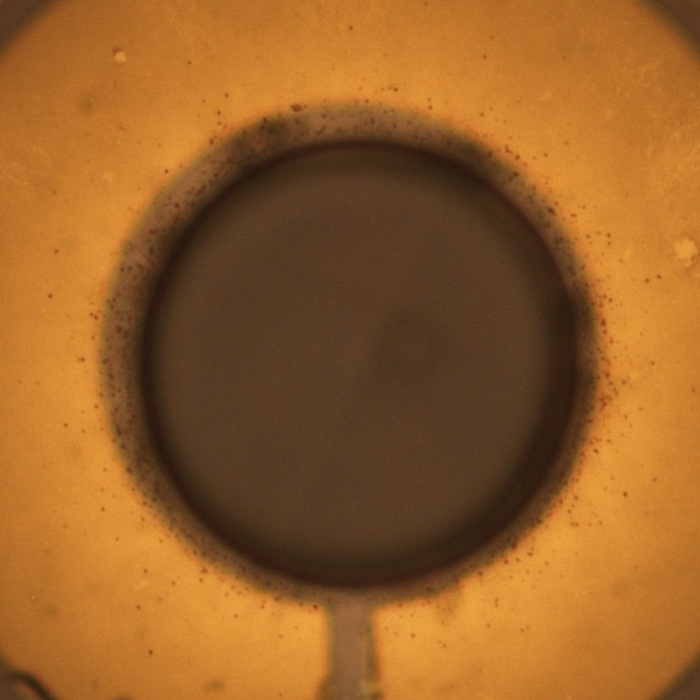
\includegraphics[width=0.4\textwidth]{figures/sample/dirt_optical_microscope.jpeg}
    \caption{An optical microscope image showing the `smut' around the trap. This `smut' is also present inside the trap.}
    \label{fig:smut-optical-microscope}
\end{SCfigure}

The current hypothesis is that this `smut' limits the free movement of the particle. This could be the case if the particle has a very low levitation height. The origin of the `smut' is likely due to oil from the roughing pump. Due to the heat of the Helmholtz coils (roughly \qty{60}{\celsius}) we think the oil evaporated or burnt and was deposited around the trap. The oil hypothesis is strengthened by the fact that we found an oil like substance on the glass of the vacuum chamber. At the time of writing the group is working on creating a new sample.

Due to the loss of levitation we were also unable to further study the dependence of the \zmode on other parameters or its Q-factor at low pressures.

\section*{Levitation height}
Changing the focus of the objective used to image the particle lets us estimate the levitation height of the particle. Based on this we noticed that the particle appears to levitate very close to the bottom of the trap. Furthermore, by changing the gradient field ($\vec{B_2}$) we did not notice any change. We think that the trap stiffness in $z$ is relatively much larger than the PCB version of the trap. A low levitation height also strengthens the hypothesis that the `smut' hindered the movement of the particle.
